\documentclass[11pt,a4paper]{article}
\usepackage[utf8]{inputenc}
\usepackage[T1]{fontenc}
\usepackage{lmodern}
\usepackage[ngerman]{babel}
\usepackage[a4paper,margin=2.5cm]{geometry}
\usepackage{amsmath,amssymb}
\usepackage{siunitx}
\DeclareSIUnit{\elementarycharge}{e^-}
\sisetup{locale=DE, per-mode=symbol}
\usepackage{booktabs}
\usepackage{tabularx}
\usepackage[section]{placeins}
\usepackage{graphicx}
\usepackage{caption}
\captionsetup{font=small,labelfont=bf}
\usepackage[hidelinks]{hyperref}

\newcommand{\Pone}{P_{\mathrm{1dB}}}
\newcommand{\Prf}{P_{\mathrm{rf}}}
\newcommand{\Ppk}{P_{\mathrm{pk}}}

\title{Benötigte Lichtleistung und Beugungseffizienz\\ des $13\times14$-Profils}
\author{Ein-Linsen-Aufbau, mit der gemessenen RF-Kette}
\date{25.~September 2026}

\begin{document}
\maketitle

\begin{abstract}
\noindent
Abschätzung für das Profil aus $13\times14$ Tönen mit \SI{1,56}{\mega\hertz}
Spanne je Achse: wie viel RF-Leistung die Kette an den AOD bringen darf, welche
Beugungseffizienz daraus folgt, wie viel Licht vor dem AOD dafür nötig ist und
was der AWG dafür ausgeben muss. Grundlage sind die Messungen vom 24./25.~09.
in \texttt{Amplifier\_characterization} und das Effizienzmodell aus
\cite{beugung}. Kurz: Die Kette ist bequem stark genug -- die bindende Grenze
ist die Schutzgrenze am AOD, nicht der Verstärker und nicht der AWG. Mit
Schroeder-Phasen liefern \SI{300}{\milli\watt} vor dem AOD etwa
\SI{209}{\milli\watt} im Profil. Die Einstellungen im aktuellen AWG-Skript
liegen allerdings um rund \SI{30}{\deci\bel} zu niedrig, und ohne Normierung
läuft der 16-Bit-Puffer über. Auf der Kameraseite ist Licht dagegen im Überfluss da: für ein Bild mit \SI{30}{\micro\second} Gate genügen Mikrowatt im Profil.
\end{abstract}

%======================================================================
\section{Die Kette und was an ihr gemessen ist}

\begin{center}\small
AWG M4i.6622-x8 $\longrightarrow$
\SI{6}{\deci\bel} Pad $+$ Limiter $+$ DC-Block $+$ \SI{190}{\mega\hertz} Tiefpass\\[2pt]
$\longrightarrow$ 5-W-Verstärker $\longrightarrow$ AOD-Achse
\end{center}

\begin{table}[htbp]
\centering\small
\begin{tabularx}{\textwidth}{@{}lXl@{}}
\toprule
Größe & Wert & Quelle\\
\midrule
AWG & M4i.6622-x8, 4 Kanäle, \SI{625}{MS/s}, 16 bit & \cite{spectrum}\\
Ausgangsamplitude & $\pm\SI{80}{\milli\volt}$ bis $\pm\SI{2,5}{\volt}$ an \SI{50}{\ohm} & \cite{spectrum}\\
Abtastrate im Skript & \SI{600}{\mega\hertz}, \SI{8}{MiS} je Kanal & Skript\\
\midrule
Kettenverstärkung $x$ (CH0) & \SI{+28,37}{\deci\bel}, Welligkeit \SI{0,03}{\deci\bel} & Messung 25.09.\\
Kettenverstärkung $y$ (CH1) & \SI{+28,64}{\deci\bel}, Welligkeit \SI{0,02}{\deci\bel} & Messung 25.09.\\
Linear geprüft bis & \SI{+0}{dBm} Eingang, \SI{+28,35}{dBm} ($\SI{684}{\milli\watt}$) Ausgang, keine Kompression & Messung 25.09.\\
Verstärker allein, Gain & \SI{+35,24}{\deci\bel} (CH0), \SI{+35,21}{\deci\bel} (CH1) & Messung 24.09.\\
Verstärker allein, $\Pone$ & \SI{+40,42}{dBm} $=\SI{11,0}{\watt}$ (CH0), \SI{+40,32}{dBm} (CH1), bei \SI{101}{\mega\hertz} & Messung 24.09.\\
\midrule
AOD & AA DTSXY-400-800, $\alpha=0{,}85$, $\beta=\SI{1,3}{\watt}$ & \cite{beugung}\\
Grenzen am AOD & $\Prf\le\SI{2}{\watt}$ (thermisch), $\Ppk\le\SI{4}{\watt}$ (Schutz) & \cite{beugung}\\
\bottomrule
\end{tabularx}
\caption{Eingangsdaten. Die \SI{6}{\deci\bel} und die Filter sitzen \emph{vor}
dem Verstärker; die Kettenverstärkung ist deshalb um \SI{6,8}{\deci\bel}
kleiner als die des Verstärkers allein, seine Ausgangsleistung aber
unverändert.}
\label{tab:kette}
\end{table}

\paragraph{Ein Vorbehalt zum $\Pone$.} Gemessen sind \SI{+40,4}{dBm}, also
\SI{11}{\watt}. Das Typenschild sagt \SI{5}{\watt} und das Datenblatt des
ZHL-03-5WF+ \SI{+36}{dBm}. Die Messung liegt \SI{4,4}{\deci\bel} darüber; das
ist mehr, als Exemplarstreuung erklärt, und wäre über die \SI{20}{\deci\bel}
des Messpads und die Analysator\-einstellungen noch einmal zu prüfen.
\textbf{Für die folgenden Zahlen ist das ohne Belang}: Schon mit dem
Datenblattwert bleibt der Verstärker die unkritischste Komponente der Kette
(Abschn.~\ref{sec:reserve}).

%======================================================================
\section{Wie viel RF-Leistung darf an den AOD?}

Für eine Achse mit dem Crestfaktor $C$ (Herleitung und Modell in
\cite{beugung}):
\begin{equation}
  \Prf = \min\!\left(\underbrace{\beta}_{\text{Sättigung}},\;
                     \underbrace{\SI{2}{\watt}}_{\text{thermisch}},\;
                     \underbrace{\frac{\SI{4}{\watt}}{C^{2}}}_{\text{AOD-Spitze}},\;
                     \underbrace{\frac{2\Pone}{C^{2}}}_{\text{Verstärker}}\right),
  \qquad
  \eta = \alpha \sin^2\!\left(\frac{\pi}{2}\sqrt{\frac{\Prf}{\beta}}\right).
  \label{eq:modell}
\end{equation}
Mit dem gemessenen $\Pone=\SI{11}{\watt}$ ist der Verstärkerterm
$2\Pone/C^2=\SI{22}{\watt}/C^2$ -- er greift erst oberhalb von $C=4{,}1$ und
spielt bei allen sinnvollen Phasensätzen keine Rolle. Es bleibt die
Schutzgrenze \SI{4}{\watt} für die Momentanspitze.

\begin{figure}[htbp]
  \centering
  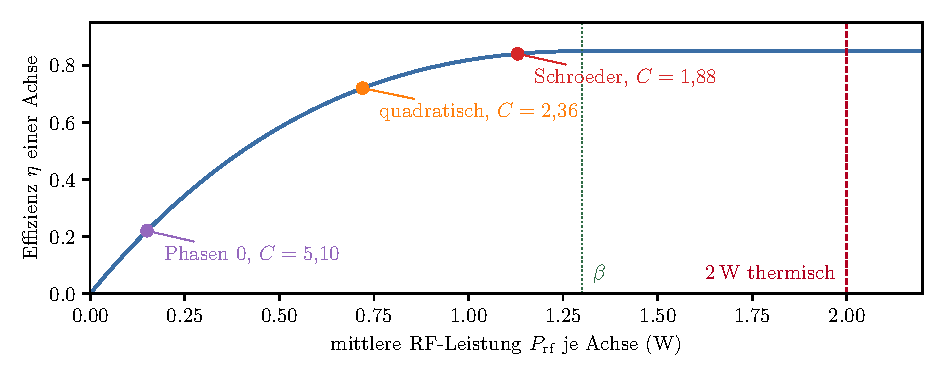
\includegraphics[width=\textwidth]{licht_eta_P.pdf}
  \caption{Effizienz einer Achse über der mittleren RF-Leistung, $\alpha=0{,}85$,
  $\beta=\SI{1,3}{\watt}$. Markiert die Arbeitspunkte, die die
  \SI{4}{\watt}-Spitzengrenze bei den jeweiligen Crestfaktoren zulässt.}
  \label{fig:etaP}
\end{figure}

\begin{table}[htbp]
\centering\small
\begin{tabular}{lccccccc}
\toprule
Tonphasen & $C_x$ & $C_y$ & $\Prf$ $x/y$ (W) & $\eta_x/\eta_y$ (\%) & $\eta_x\eta_y$ & im Profil & je Spot\\
\midrule
alle 0            & 5,10 & 5,29 & 0,15 / 0,14 & 22 / 21 & \SI{4,7}{\percent}  & \SI{14}{\milli\watt}  & \SI{0,08}{\milli\watt}\\
Schroeder         & 1,88 & 1,94 & 1,13 / 1,06 & 84 / 83 & \SI{69,8}{\percent} & \SI{209}{\milli\watt} & \SI{1,15}{\milli\watt}\\
Kitayoshi         & 1,88 & 1,94 & 1,13 / 1,06 & 84 / 83 & \SI{69,8}{\percent} & \SI{209}{\milli\watt} & \SI{1,15}{\milli\watt}\\
$2\pi n(n-1)/(N-1)$ & 2,36 & 2,16 & 0,72 / 0,85 & 72 / 78 & \SI{55,8}{\percent} & \SI{167}{\milli\watt} & \SI{0,92}{\milli\watt}\\
symm.\ optimiert ($C\le1{,}9$) & 1,89 & 1,89 & 1,12 / 1,12 & 84 / 84 & \SI{70,4}{\percent} & \SI{211}{\milli\watt} & \SI{1,16}{\milli\watt}\\
\bottomrule
\end{tabular}
\caption{$13\times14$ Töne, \SI{300}{\milli\watt} vor dem AOD, 182 Spots. In
jeder Zeile begrenzt die \SI{4}{\watt}-Spitze am AOD. \glqq je Spot\grqq{} ist
das Mittel; die Randtöne tragen etwas weniger.}
\label{tab:phasen}
\end{table}

%======================================================================
\section{Benötigte Lichtleistung vor dem AOD}

Aus $P_\mathrm{Profil}=P_\mathrm{in}\,\eta_x\eta_y$ folgt unmittelbar
$P_\mathrm{in}=P_\mathrm{Profil}/(\eta_x\eta_y)$:

\begin{table}[htbp]
\centering\small
\begin{tabular}{lcccc}
\toprule
 & \multicolumn{4}{c}{nötige Leistung vor dem AOD}\\
\cmidrule(lr){2-5}
Tonphasen & \SI{50}{\milli\watt} & \SI{100}{\milli\watt} & \SI{150}{\milli\watt} & \SI{200}{\milli\watt} im Profil\\
\midrule
Schroeder / Kitayoshi & \SI{72}{\milli\watt} & \SI{143}{\milli\watt} & \SI{215}{\milli\watt} & \SI{287}{\milli\watt}\\
symm.\ optimiert      & \SI{71}{\milli\watt} & \SI{142}{\milli\watt} & \SI{213}{\milli\watt} & \SI{284}{\milli\watt}\\
$2\pi n(n-1)/(N-1)$   & \SI{90}{\milli\watt} & \SI{179}{\milli\watt} & \SI{269}{\milli\watt} & \SI{358}{\milli\watt}\\
alle 0                & \SI{1,06}{\watt}     & \SI{2,13}{\watt}      & \SI{3,19}{\watt}      & \SI{4,26}{\watt}\\
\bottomrule
\end{tabular}
\caption{Ohne die Optik hinter den AODs. Die Transmission dort und die
Verluste der Abbildung kommen noch dazu.}
\label{tab:bedarf}
\end{table}

Mit den vorhandenen \SI{300}{\milli\watt} sind also alle Ziele bis etwa
\SI{200}{\milli\watt} im Profil erreichbar, solange der Crestfaktor unter
etwa~2 bleibt. Mit Phasen null ist selbst \SI{50}{\milli\watt} nicht erreichbar.

%======================================================================
\section{Was der AWG liefern muss}
\label{sec:reserve}

Die Kette verstärkt um $G=\SI{28,37}{\deci\bel}$ ($x$) bzw.
$\SI{28,64}{\deci\bel}$ ($y$), also um den Faktor 687 bzw.~731 in der Leistung.
Für die Spitzenspannung am AWG-Ausgang an \SI{50}{\ohm} gilt mit
$\Ppk=C^2\Prf$
\begin{equation}
  V_\mathrm{pk}^\mathrm{AWG} = \sqrt{\frac{2R\,\Ppk}{2\,G}}
  = \sqrt{\frac{R\,C^{2}\Prf}{G}} .
  \label{eq:vpk}
\end{equation}
Da in allen Zeilen von Tab.~\ref{tab:phasen} dieselbe Spitzenleistung
$\Ppk=\SI{4}{\watt}$ ausgeschöpft wird, ist die nötige Spitzenspannung immer
dieselbe:
\begin{equation*}
  V_\mathrm{pk}^\mathrm{AWG} = \SI{0,54}{\volt}\ (x), \qquad \SI{0,52}{\volt}\ (y),
  \qquad\text{gegen \SI{2,5}{\volt} Maximum: \SI{13,3}{\deci\bel} Reserve.}
\end{equation*}
Die mittlere Leistung am AWG liegt dabei bei \SI{+2,2}{dBm} ($x$) bzw.
\SI{+1,6}{dBm} ($y$) -- innerhalb des Bereichs, in dem die Kette am 25.09.\
nachweislich linear war (bis \SI{0}{dBm} Eingang gemessen, \SI{2}{\deci\bel}
darunter).

\paragraph{Reserve des Verstärkers.} Die Spitzenhüllkurvenleistung am
Verstärkerausgang ist $\mathrm{PEP}=\Ppk/2=\SI{2,0}{\watt}=\SI{33,0}{dBm}$,
also \SI{7,4}{\deci\bel} unter dem gemessenen $\Pone$ und \SI{3}{\deci\bel}
unter dem Datenblattwert \SI{+36}{dBm}. Die Kette arbeitet damit in beiden
Lesarten linear.

\begin{figure}[htbp]
  \centering
  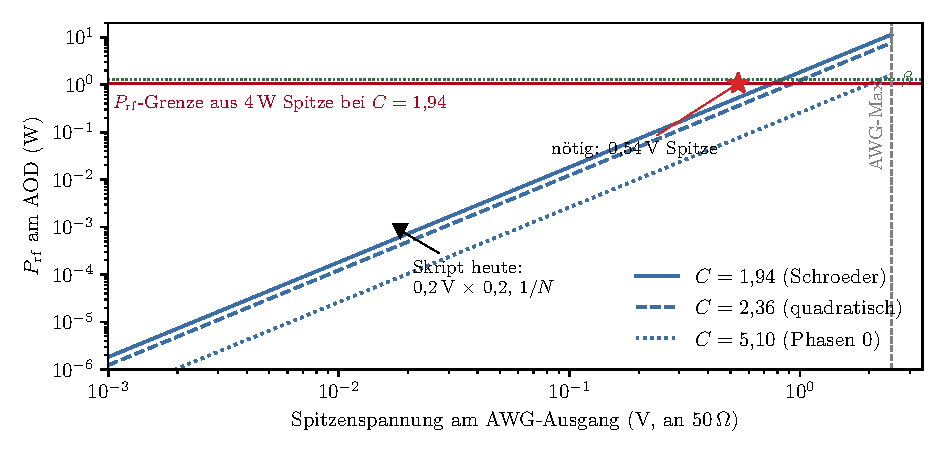
\includegraphics[width=\textwidth]{licht_P_awg.pdf}
  \caption{Mittlere RF-Leistung am AOD über der Spitzenspannung des AWG,
  $G=\SI{28,37}{\deci\bel}$. Stern: der nötige Arbeitspunkt. Dreieck: was die
  Einstellungen im aktuellen Skript ergeben. Gestrichelt rechts das
  AWG-Maximum von \SI{2,5}{\volt}.}
  \label{fig:awg}
\end{figure}

%======================================================================
\section{Abgleich mit dem AWG-Skript}

Zwei Punkte im aktuellen \texttt{2\_gen\_single\_2ch.py} stehen dem entgegen.

\paragraph{1. Der Pegel ist etwa \SI{30}{\deci\bel} zu klein.} Gesetzt sind
\texttt{channels.amp(0.2 V)} und ein digitaler Faktor $0{,}2$, und
\texttt{generate\_signal} normiert zusätzlich mit $1/N$. Für 13 Töne mit
$C=2{,}36$ ist der Effektivwert des normierten Signals $1/\sqrt{2N}=0{,}196$,
also
\begin{equation*}
  V_\mathrm{rms} = \SI{0,2}{\volt}\cdot 0{,}2 \cdot 0{,}196 = \SI{7,8}{\milli\volt}
  \;\Rightarrow\; P_\mathrm{AWG} = \SI{-29,1}{dBm}
  \;\Rightarrow\; \Prf = \SI{0,85}{\milli\watt},
\end{equation*}
und damit $\eta\approx\SI{0,14}{\percent}$ je Achse, also etwa
$2\cdot10^{-6}$ des Lichts im Profil. Nötig ist rund der Faktor 1000 in der
Leistung.

\paragraph{2. \texttt{generate\_signal2} normiert gar nicht.} Dort werden $N$
Sinus mit Amplitude~1 summiert und mit $2^{15}\cdot0{,}2$ skaliert. Für 13 Töne
mit quadratischen Phasen ist die Spitze
$C\sqrt{N/2}=6{,}0$, also $6{,}0\cdot6553=39\,500 > 32\,767$: Der
\texttt{int16}-Puffer läuft über und klappt um -- das Signal ist dann nicht
mehr das gerechnete. Bei den bisher benutzten 3 und 4 Tönen fiel das nicht auf.

\paragraph{Empfehlung.} Das Sample-Array auf seine eigene Spitze normieren und
den Pegel allein über \texttt{channels.amp()} stellen:
\begin{equation*}
  \texttt{signal} \;\rightarrow\; 0{,}95\cdot 2^{15}\cdot\frac{s(t)}{\max_t |s(t)|},
  \qquad
  \texttt{channels.amp} = \frac{V_\mathrm{pk}^\mathrm{AWG}}{0{,}95}
  \approx \SI{0,57}{\volt}\ (x),\ \SI{0,55}{\volt}\ (y).
\end{equation*}
Dann ist die Aussteuerung des DAC unabhängig von Tonzahl und Phasensatz, und
die Spitzenleistung am AOD steht auf den erlaubten \SI{4}{\watt}. Wer die
\SI{4}{\watt}-Schutzgrenze nicht ausreizen will, senkt allein
\texttt{channels.amp} -- die Effizienz folgt Gl.~\eqref{eq:modell}, siehe
Abb.~\ref{fig:etaP}.

%======================================================================
\section{Was die Kamera braucht}

Die Abschnitte oben sagen, wie viel Licht \emph{ankommt}. Ob ein Pixel davon
genug bekommt, ist eine andere Frage -- und sie dreht die Richtung um.

Bei 1:1-Abbildung f\"allt auf ein Pixel von \SI{1,45}{\micro\meter} Kantenl\"ange
der Bruchteil
\begin{equation}
  \frac{A_\mathrm{px}}{A_\mathrm{Plateau}} = 2{,}36\cdot10^{-4}
  \label{eq:pxanteil}
\end{equation}
der Profilleistung (Plateaufl\"ache \SI{8165}{\micro\meter\squared}, aus dem
Zeitmittel des $13\times14$-Profils). Mit dem Gate der L\"ange $t_g$, der
Quanteneffizienz $\mathrm{QE}$ und $h\nu$ bei \SI{795}{\nano\meter} sind das
\begin{equation}
  N_{\mathrm{e}^-} = \frac{P_\mathrm{Profil}\,\cdot 2{,}36\cdot10^{-4}\cdot t_g\cdot \mathrm{QE}}{h\nu}
  \qquad\text{Elektronen je Plateau-Pixel.}
  \label{eq:elektronen}
\end{equation}

\begin{table}[htbp]
\centering\small
\begin{tabular}{lccl}
\toprule
$P_\mathrm{Profil}$ (Puls) & $P_\mathrm{in}$ vor dem AOD & $N_{\mathrm{e}^-}$ & Bewertung\\
\midrule
\SI{0,06}{\micro\watt} & \SI{0,08}{\micro\watt} & 500  & SNR des Hubs $\approx10$, untere Grenze\\
\SI{0,24}{\micro\watt} & \SI{0,34}{\micro\watt} & 2000 & SNR $\approx20$, guter Arbeitspunkt\\
\SI{0,47}{\micro\watt} & \SI{0,67}{\micro\watt} & 4000 & im hellen Moment ($+\SI{44}{\percent}$) knapp\\
\SI{1}{\micro\watt}    & \SI{1,4}{\micro\watt}  & 8500 & ges\"attigt\\
\bottomrule
\end{tabular}
\caption{$t_g=\SI{30}{\micro\second}$, 1:1, $\mathrm{QE}=0{,}30$,
S\"attigungsladung \SI{6000}{\elementarycharge} angenommen; $P_\mathrm{in}$ mit
$\eta_x\eta_y=\SI{69,8}{\percent}$ (Schroeder-Phasen).}
\label{tab:kamera}
\end{table}

\begin{figure}[htbp]
  \centering
  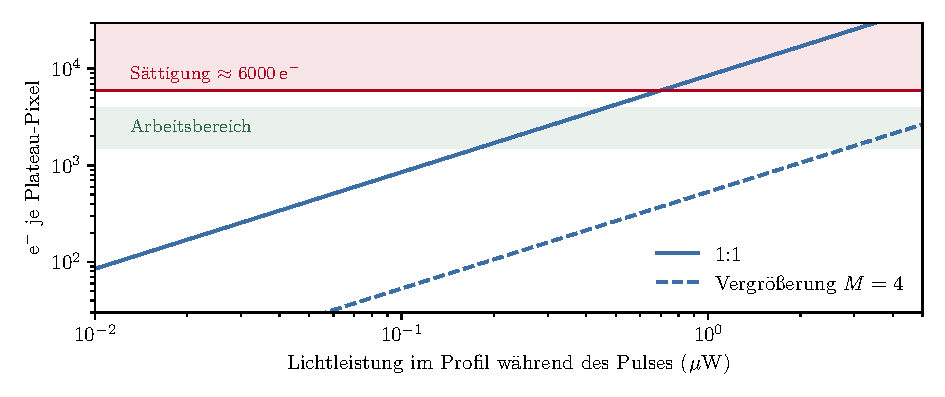
\includegraphics[width=\textwidth]{licht_kamera.pdf}
  \caption{Elektronen je Plateau-Pixel nach Gl.~\eqref{eq:elektronen}. Der
  gr\"une Streifen ist der Arbeitsbereich: gen\"ugend Abstand zum Ausleserauschen
  und noch Platz f\"ur den Hub der Schwebung von \SI{44}{\percent}.}
  \label{fig:kamera}
\end{figure}

\paragraph{Die Folgerung.} Gebraucht werden \emph{Mikrowatt}, nicht Milliwatt.
Von den \SI{209}{\milli\watt}, die bei \SI{300}{\milli\watt} Eingang im Profil
ank\"amen, m\"usste um rund \SI{58}{\deci\bel} abgeschw\"acht werden. Die
Lichtleistung ist f\"ur diese Messung also keine Randbedingung; entscheidend ist,
\emph{einstellen} zu k\"onnen, so dass das Plateau im Einzelbild bei etwa einem
Drittel bis der H\"alfte der Vollaussteuerung liegt.

\paragraph{Wie die Zahlen skalieren.}
\begin{itemize}
\item \textbf{Vergr\"o\ss{}erung $M$:} ein Pixel sammelt $M^{-2}$ so viel. Mit
  $M=4$, sinnvoll f\"ur saubere Spotprofile, werden aus \SI{0,24}{\micro\watt}
  rund \SI{3,8}{\micro\watt}.
\item \textbf{Pulsl\"ange:} linear. Bei \SI{10}{\micro\second} das Dreifache --
  und k\"urzer als etwa \SI{10}{\micro\second} ist wegen der Schall-Laufzeit im
  AOD (\SI{5,4}{\micro\second}) ohnehin nicht sinnvoll.
\item \textbf{QE und S\"attigungsladung} sind Annahmen f\"ur den IMX415 bei
  \SI{795}{\nano\meter}; beide sind aus der QE-Kurve bzw.\ dem Datenblatt zu
  best\"atigen. Ein Faktor~2 dort verschiebt alle Zahlen um denselben Faktor.
\item \textbf{Ausleserauschen} (wenige \si{\elementarycharge}) spielt im
  Arbeitsbereich keine Rolle; es dominiert das Schrotrauschen mit
  $1/\sqrt{N_{\mathrm{e}^-}}$.
\end{itemize}

\section{Vorbehalte}

\begin{itemize}
\item \textbf{Der Limiter} in der Filterkette begrenzt die Spitzenspannung,
  und genau die Spitze ist bei einem Mehrtonsignal groß. Seine Schwelle ist
  hier nicht bekannt; liegt sie unter der oben genannten Spitze, schneidet er
  die Rephasierungsspitzen ab und erzeugt Intermodulation. Das ist der
  Punkt, der als Nächstes gemessen gehört -- zum Beispiel mit zwei Tönen
  wachsender Amplitude am Spektrumanalysator.
\item \textbf{$\beta$ ist nicht an diesem Gerät gemessen.} Mit
  $\beta=\SI{1,8}{\watt}$ statt \SI{1,3}{\watt} fällt die Effizienz bei
  Schroeder-Phasen von \SI{84}{\percent} auf \SI{76}{\percent} je Achse
  (\SI{170}{\milli\watt} statt \SI{209}{\milli\watt} im Profil) \cite{beugung}.
\item \textbf{Intermodulation im AOD} ist nicht enthalten; bei 40 Tönen sind
  \SI{-18}{\deci\bel} gemessen, bei 10 Tönen nichts Sichtbares \cite{beugung}.
  Bei 13 bzw.\ 14 Tönen ist ein Verlust im Prozentbereich zu erwarten.
\item \textbf{Die \SI{4}{\watt}-Spitzengrenze} ist Laborpraxis, kein
  Datenblattwert. Sie ist hier die einzige bindende Grenze -- wer sie ändert,
  ändert alle Zahlen dieses Dokuments.
\item Optik hinter den AODs, Frequenzgang von $\alpha$ und $\beta$ und der
  Kopplungsterm der gekreuzten AODs sind nicht enthalten.
\end{itemize}

\begin{thebibliography}{9}
\bibitem{beugung} \emph{Beugungseffizienz der gekreuzten AODs in Abhängigkeit
  vom Crestfaktor}, interne Ausarbeitung, 22.~September 2026.
\bibitem{messung} Messreihen \texttt{5W\_CH0/CH1\_with\_preamp} (24.09.2026) und
  \texttt{5W\_CH0/CH1\_AODconfig(6dB)} (25.09.2026),
  \texttt{Amplifier\_characterization}.
\bibitem{spectrum} Spectrum Instrumentation, M4i.6622-x8,
  \url{https://spectrum-instrumentation.com/products/details/M4i6622-x8.php}.
\bibitem{testsheet} AA Opto-Electronic, Test Sheet DTSXY-400-800, S/N
  3001-O211386 (12.04.2022).
\end{thebibliography}

\end{document}
